\begin{figure}[h!]
	\centering
	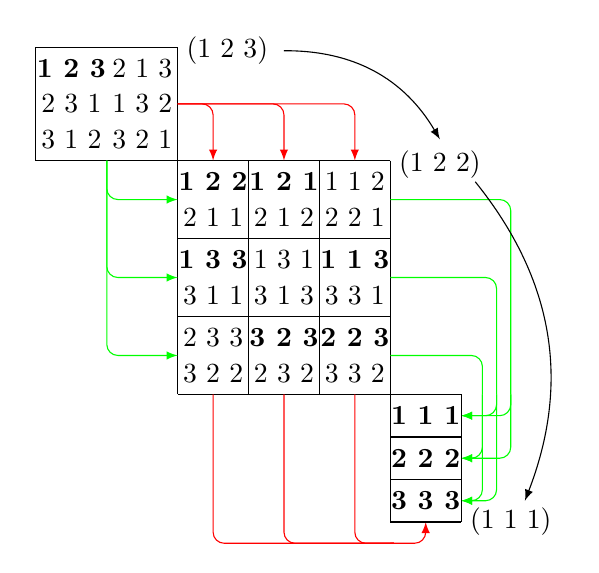
\begin{tikzpicture}[scale = 0.9]
	\tikzstyle{fleche}=[->,>=latex,rounded corners=4pt]
	\node at (2.2,0.25){$\jc$(1 2 3)};
	\node[font = \bfseries] at (0,0){1 2 3};
	\node at (0,-1/2){2 3 1};
	\node at (0,-1){3 1 2};
	\node at (1,0){2 1 3};
	\node at (1,-1/2){1 3 2};
	\node at (1,-1){3 2 1};
	
	
	\draw[black] (-.5,.3) to (1.5, .3);
	\draw[black] (-.5,.3) to (-.5, -1.3);
	\draw[black] (1.5,.3) to (1.5, -4.6);
	\draw[black] (-.5,-1.3) to (4.5, -1.3);
	
	\draw[fleche, red] (1.5,-1/2) -| (2, -1.3);
	\draw[fleche, red] (1.5,-1/2) -| (3, -1.3);
	\draw[fleche, red] (1.5,-1/2) -| (4, -1.3);
	\draw[fleche, green] (.5,-1.3) |- (1.5, -1.85);
	\draw[fleche, green] (.5,-1.3) |- (1.5, -2.95);
	\draw[fleche, green] (.5,-1.3) |- (1.5, -4.05);
	
	\node at (5.2,-1.6+0.25){$\jc$(1 2 2)};
	\draw[->,>=latex, bend left] (3,0.25) to (5.2,-1);
	\node[font = \bfseries] at (2,-1.6){1 2 2};
	\node at (2,-2.1){2 1 1};
	\node[font = \bfseries] at (3,-1.6){1 2 1};
	\node at (3,-2.1){2 1 2};
	\node at (4,-1.6){1 1 2};
	\node at (4,-2.1){2 2 1};
	
	\draw[black] (1.5, -2.4) to (4.5, -2.4);
	
	\node[font = \bfseries] at (2,-2.7){1 3 3};
	\node at (2,-3.2){3 1 1};
	\node at (3,-2.7){1 3 1};
	\node at (3,-3.2){3 1 3};
	\node[font = \bfseries] at (4,-2.7){1 1 3};
	\node at (4,-3.2){3 3 1};
	
	\draw[black] (1.5, -3.5) to (4.5, -3.5);
	
	\node at (2,-3.8){2 3 3};
	\node at (2,-4.3){3 2 2};
	\node[font = \bfseries] at (3,-3.8){3 2 3};
	\node at (3,-4.3){2 3 2};
	\node[font = \bfseries] at (4,-3.8){2 2 3};
	\node at (4,-4.3){3 3 2};
	
	\draw[black] (1.5, -4.6) to (5.5, -4.6);
	\draw[black] (2.5, -1.3) to (2.5, -4.6);
	\draw[black] (3.5, -1.3) to (3.5, -4.6);
	\draw[black] (4.5, -1.3) to (4.5, -6.4);
	
	\draw[rounded corners=4pt, red] (2, -4.6) |- (4.55, -6.7);
	\draw[rounded corners=4pt, red] (3, -4.6) |- (4.55, -6.7);
	\draw[rounded corners=4pt, red] (4, -4.6) |- (4.55, -6.7);
	\draw[fleche, red] (4.5, -6.7) -| (5, -6.4);
	\draw[rounded corners=4pt, green] (4.5, -1.85) -| (6.2, -4.6);
	\draw[fleche, green] (6.2, -4.6) |- (5.5, -4.9);
	\draw[fleche, green] (6.2, -4.6) |- (5.5, -5.5);
	\draw[rounded corners=4pt, green] (4.5, -2.95) -| (6, -4.6);
	\draw[fleche, green] (6, -4.6) |- (5.5, -4.9);
	\draw[fleche, green] (6, -4.6) |- (5.5, -6.1);
	\draw[rounded corners=4pt, green] (4.5, -4.05) -| (5.8, -4.6);
	\draw[fleche, green] (5.8, -4.6) |- (5.5, -6.1);
	\draw[fleche, green] (5.8, -4.6) |- (5.5, -5.5);
	
	\node at (6.2,-6.4){$\jc$(1 1 1)};
	\draw[->,>=latex, bend left] (5.7,-1.6) to (6.4,-6.1);
	\node[font = \bfseries] at (5, -4.9){1 1 1};
	\draw[black] (4.5, -5.2) to (5.5, -5.2);
	\node[font = \bfseries] at (5, -5.5){2 2 2};
	\draw[black] (4.5, -5.8) to (5.5, -5.8);
	\node[font = \bfseries] at (5, -6.1){3 3 3};
	
	\draw[black] (5.5, -4.6) to (5.5, -6.4);
	\draw[black] (4.5, -6.4) to (5.5, -6.4);
	
	\end{tikzpicture}
	\caption[Green relations in $T_3$.]{Green relations in $T_3$. \\ {\small Each block is a $\jc$-class, each line is a $\rc$-class, each column a $\lc$-class and each case an $\hc$-class. The red, green and black arrows represent the $\lc$, $\rc$ and $\jc$-order respectively.}}
\end{figure}